\documentclass[11pt]{beamer}
\usetheme{default}
\usecolortheme{beaver}
\usepackage{fancyvrb}
\usepackage{eurosym}
\usepackage[utf8]{inputenc}
\DeclareUnicodeCharacter{20AC}{\euro}
\usepackage{pmboxdraw}
\usepackage[english]{babel}
\usepackage{amsmath}
\usepackage{amsfonts}
\usepackage{amssymb}
\usepackage{listings}
\usepackage{mathtools}
\DeclarePairedDelimiter{\ceil}{\lceil}{\rceil}
\usepackage{caption}
\usepackage{hyperref}
\hypersetup{
    colorlinks=true,
    linkcolor=blue,
    filecolor=magenta,      
    urlcolor=cyan,
}
\captionsetup[figure]{labelformat=empty}
\author{Mattia Bacarella - 928345\\
		Francesco Corda - 920212\\
		Davide Damato - 920616\\
		Luciano Franchin - 921093\\
		Luca Massini - 945027}
\title{Pricing and Advertising}
\subtitle{Project for the Data Intelligence Application Class\\
		PoliMi 2019-2020}
		
\usepackage{xcolor}

\definecolor{codegreen}{rgb}{0,0.6,0}
\definecolor{codegray}{rgb}{0.5,0.5,0.5}
\definecolor{codepurple}{rgb}{0.58,0,0.82}
\definecolor{backcolour}{rgb}{0.95,0.95,0.92}

\lstdefinestyle{mystyle}{
    backgroundcolor=\color{backcolour},   
    commentstyle=\color{codegreen},
    keywordstyle=\color{magenta},
    numberstyle=\tiny\color{codegray},
    stringstyle=\color{codepurple},
    basicstyle=\ttfamily\footnotesize,
    breakatwhitespace=false,         
    breaklines=true,                 
    captionpos=b,                    
    keepspaces=true,                 
    numbers=left,                    
    numbersep=5pt,                  
    showspaces=false,                
    showstringspaces=false,
    showtabs=false,                  
    tabsize=2
}

\lstset{
	style=mystyle,
	escapechar={|}
	}

\makeatletter
\let\@@magyar@captionfix\relax
\makeatother
\begin{document}

\begin{frame}
\titlepage
\end{frame}

%\begin{frame}
%\tableofcontents
%\end{frame}

\begin{frame}{Objective of the Project}
\textit{The goal is to model a scenario in which a seller exploits advertising tools to attract more and more users to its website, thus increasing the number of possible buyers. The seller needs to learn simultaneously the conversion rate and the number of users the advertising tools can attract.}
\end{frame}

\begin{frame}[fragile]{Project Structure}
\begin{itemize}
\item Repository: \url{https://github.com/francescocorda/dia-project}
\item Structure:
\begin{verbatim}
dia_project
 ├── assignment_2
 ├── assignment_3
 ├── assignment_4
 ├── assignment_5
 ├── assignment_6
 ├── assignment_7
 ├── data
 └── utils
\end{verbatim}
\item The project is organized in modules, one for each assignment. To execute the code and reproduce our results, run the file assignment\_x.py in each module.
\end{itemize}
\end{frame}

\begin{frame}{Project Roadmap}
After the definition of the working environment, the project can be divided in three main sections:
\begin{itemize}
\item a first part dedicated to advertising the product, with the goal of maximizing the traffic (expressed as number of clicks) directed to our web page
\item a second part dedicated to the pricing, with the goal of finding the optimal selling point to obtain the highest revenue
\item a third part in which the actions are combined, the algorithm learns simultaneously to advertise and sell
\end{itemize}
\begin{figure}[hbtp]
\centering
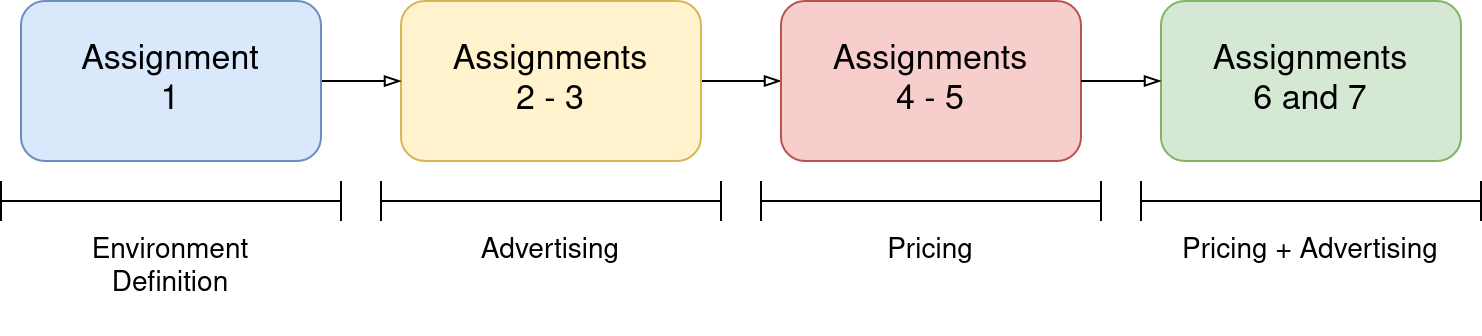
\includegraphics[width=\textwidth]{images/roadmap.png}
\end{figure}

\end{frame}

\begin{frame}{Assignment 1}
\textit{Imagine one product to sell:
\begin{itemize}
\item three classes of users, where, for every user, we can observe the values of two binary features (feel free to choose the features and their domains);
\item the conversion rate curve of each class of users;
\item three subcampaigns, each with a different ad, to advertise the product, and each targeting a different class of users;
\item there are three abrupt phases;
\item for every abrupt phase and for every subcampaign, the probability distribution over the daily number of clicks for every value of budget allocated to that subcampaign.
\end{itemize}}
\end{frame}

\begin{frame}{Assignment 1 - The Product}
We decided to analyze the pricing and the advertising of a \textbf{gym membership}, a product that presents the following properties:
\begin{itemize}
\item it's a well-known and established item, used by a vast and diversified population of users
\item it's a highly customizable product, that allows for different advertising campaigns and price offers for different classes of users
\item it's strongly affected by seasonality during the year
\end{itemize}
\end{frame}

\begin{frame}{Assignment 1 - Users}
The users are characterized with a set of 2 binary features, namely:
\begin{itemize}
\item Age = \{Under 40, Over 40\}
\item Fitness Level = \{Novice, Experienced\}
\end{itemize}
We decided to focus on the following 3 classes generated by the features:
\begin{itemize}
\item (Under 40, Novice)
\item (Under 40, Experienced)
\item (Over 40, Experienced)
\end{itemize}
We excluded the class of (Over 40, Novice) users because of the online nature of our advertising campaign: an adult person which is not already interested in fitness is less likely to look on the internet for arguments related to our campaign.
\end{frame}

\begin{frame}{Assignment 1 - Conversion Rate Curves}
Given a domain for the prices of a gym subscription that ranges from € 0 to € 100, we identified 3 curves with the following characteristics:
\begin{itemize}
\item all curves present a monotonically decreasing trend, starting from a conversion rate of 1 and ending towards 0
\item to add realism to the curves, the conversion rates maintain values close to 1 until a minimum price threshold is reached  
\end{itemize}
The classes differ in their sensitivity to price increases, according to principles that a novice is in general less interested in an expensive item than an expert and that an adult has on average an higher purchasing power than a young person.

\end{frame}

\begin{frame}{Assignment 1 - (Under 40, Novice) class}
\begin{figure}[hbtp]
\centering
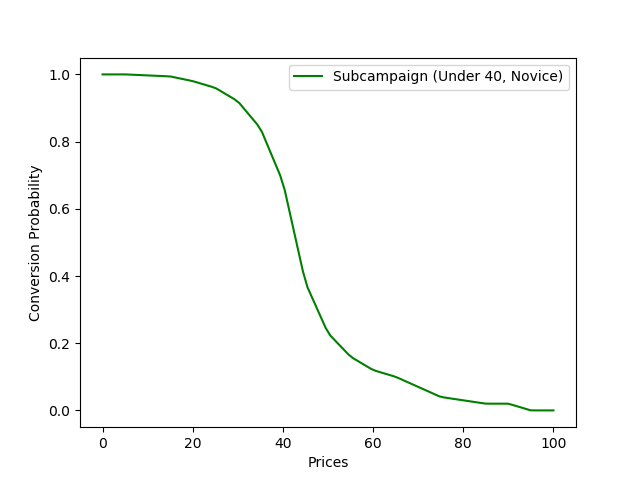
\includegraphics[width=0.8\textwidth]{images/demand_curve_2.png}
\caption{Fast decrease.}
\end{figure}
\end{frame}

\begin{frame}{Assignment 1 - (Under 40, Experienced) class}
\begin{figure}[hbtp]
\centering
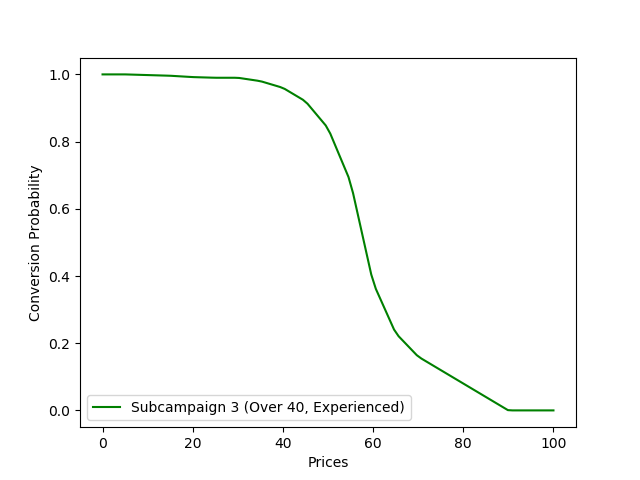
\includegraphics[width=0.8\textwidth]{images/demand_curve_3.png}
\caption{Intermediate decrease.}
\end{figure}
\end{frame}

\begin{frame}{Assignment 1 - (Over 40, Experienced) class}
\begin{figure}[hbtp]
\centering
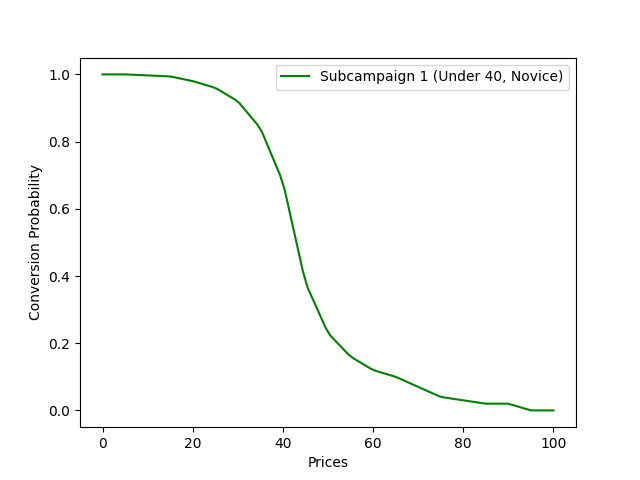
\includegraphics[width=0.8\textwidth]{images/demand_curve_1.png}
\caption{Slow decrease.}
\end{figure}
\end{frame}

\begin{frame}{Assignment 1 - Subcampaigns}
Each class is the object of interest of a web marketing subcampaign.
One goal of the project is the allocation of the advertising daily budget to maximize the total number of clicks. 
To do this, we identified 3 curves that describe this number as a function of the portion of the budget allocated to the campaign (from 0\% to 100\%).\\
All curves increase monotonically with the budget spent, until they reach a plateau in which allocating more money to the campaign does not produce results.\\
The campaigns differ for the maximum number of clicks reached and the sensitivity to the allocated budget.

\end{frame}

\begin{frame}{Assignment 1 - Subcampaign 1}
\begin{figure}[hbtp]
\centering
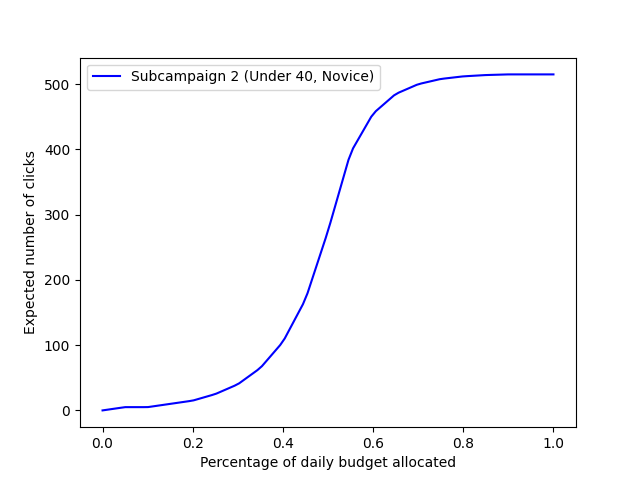
\includegraphics[width=0.8\textwidth]{images/subcampaign_2.png}
\caption{Fast increase, medium value plateau.}
\end{figure}
\end{frame}

\begin{frame}{Assignment 1 - Subcampaign 2}
\begin{figure}[hbtp]
\centering
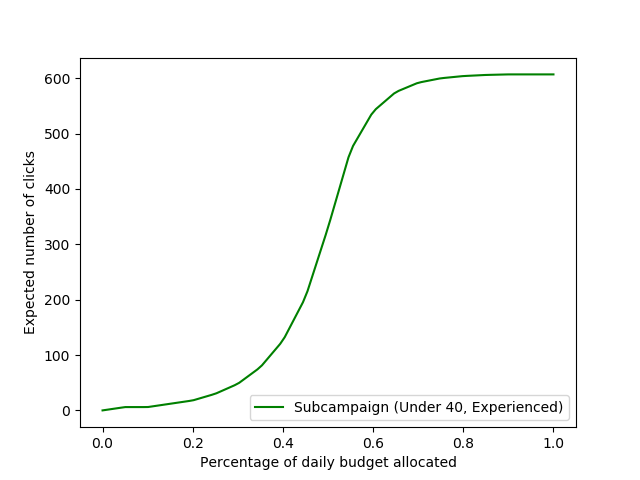
\includegraphics[width=0.8\textwidth]{images/subcampaign_3.png}
\caption{Fast increase, high value plateau.}
\end{figure}
\end{frame}

\begin{frame}{Assignment 1 - Subcampaign 3}
\begin{figure}[hbtp]
\centering
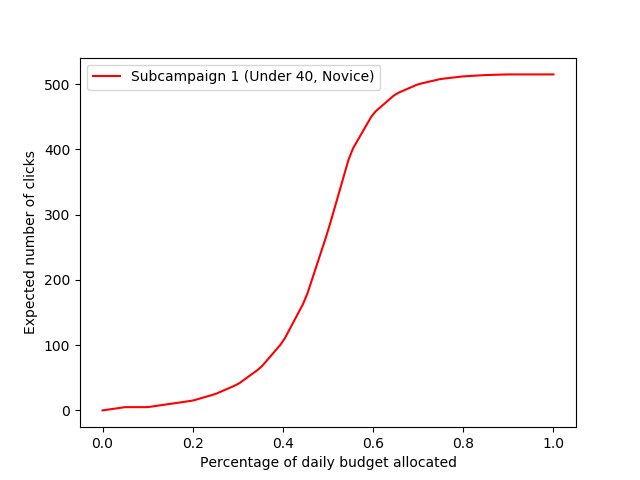
\includegraphics[width=0.8\textwidth]{images/subcampaign_1.png}
\caption{Slow increase, small value plateau.}
\end{figure}
\end{frame}

\begin{frame}{Assignment 1 - Abrupt Phases}
We identified 3 abrupt phases influenced by the seasonality that characterizes gym subscriptions during a year:
\begin{itemize}
\item [1.] [January-April], the ``New Year's Resolutions" phase, it's the period with the highest interest
\item [2.] [May-August], the ``Swimsuit Season" phase, in which the least number of users is attracted
\item [3.] [September-December], the ``Back to Normal" phase, with an intermediate level of activity 
\end{itemize}
Each period has the same length of 4 months and is denoted by almost-stationary behaviors of the users for its duration. The classes are influenced by the abrupt phases in different measures.
\end{frame} 

\begin{frame}{Assignment 1 - Subcampaign 1, Abrupt Phases}
\begin{figure}[hbtp]
\centering
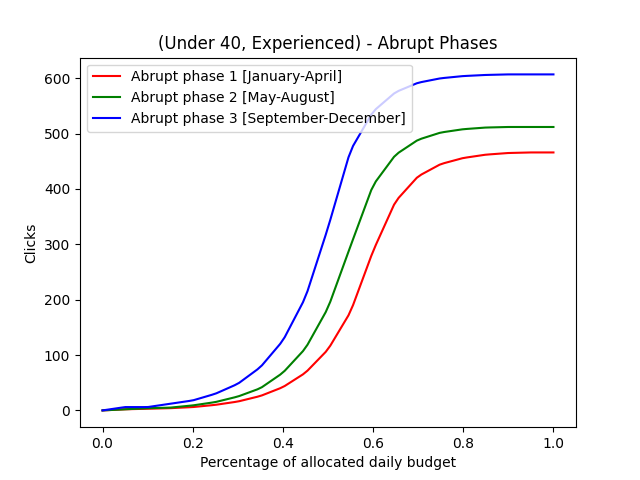
\includegraphics[width=0.8\textwidth]{images/subcampaign_2_abrupt_phases.png}
\caption{The (Under 40, Novice) class has a medium interest in the product during the year, with a significant drop during Summer.}
\end{figure}
\end{frame}

\begin{frame}{Assignment 1 - Subcampaign 2, Abrupt Phases}
\begin{figure}[hbtp]
\centering
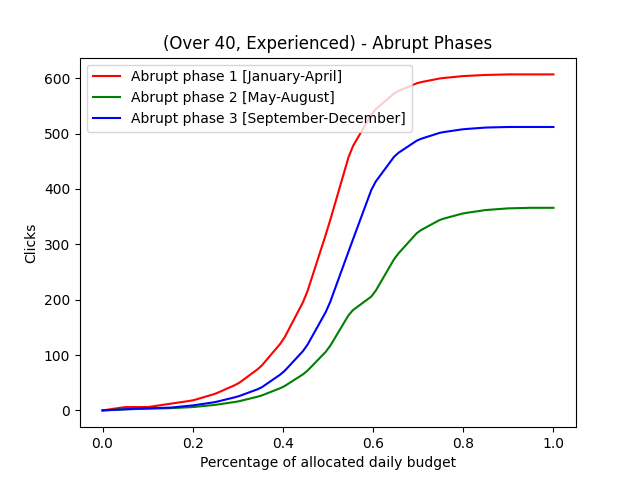
\includegraphics[width=0.8\textwidth]{images/subcampaign_3_abrupt_phases.png}
\caption{The (Under 40, Experienced) class has the highest interest in product in all phases.}
\end{figure}
\end{frame}

\begin{frame}{Assignment 1 - Subcampaign 3, Abrupt Phases}
\begin{figure}[hbtp]
\centering
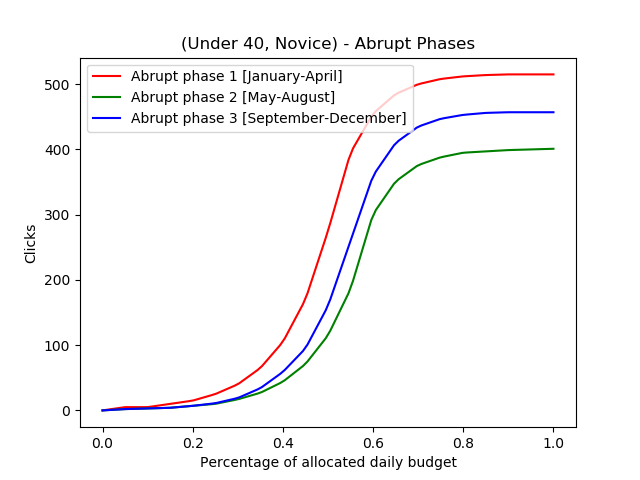
\includegraphics[width=0.8\textwidth]{images/subcampaign_1_abrupt_phases.png}
\caption{The (Over 40, Experienced) class has the lowest interest in the product, but is the least affected by seasonality.}
\end{figure}
\end{frame}

\begin{frame}{Assignment 2}
\textit{Design a combinatorial bandit algorithm to optimize the budget allocation over the three subcampaigns to maximize the total number of clicks when, for simplicity, there is only one phase. Plot the cumulative regret.}
\end{frame}

\begin{frame}[fragile]{Assignment 2 - Pseudocode}
\begin{lstlisting}
|\color{cyan}initialize| click envs
|\color{cyan}for| exp |\color{cyan}in| n_experiments:
  |\color{cyan}initialize| gp-ts learners
  |\color{cyan}for| t |\color{cyan}in| time_horizon:
    draw samples for each subcampaign
    find super-arm by solving knapsack problem
    |\color{cyan}pull| arms given by super-arm
    |\color{cyan}update| gp-ts learners
|\color{cyan}calculate| clairvoyant value
|\color{cyan}plot| rewards and regrets
\end{lstlisting}
\end{frame}

\begin{frame}{Assignment 2 - Experiments}
Setting parameters:
\begin{itemize}
\item T = 365
\item Number of arms = 21
\item Number of experiments = 50
\end{itemize}
\end{frame}

\begin{frame}{Assignment 2 -  Cumulative Regret}
\begin{figure}[hbtp]
\centering
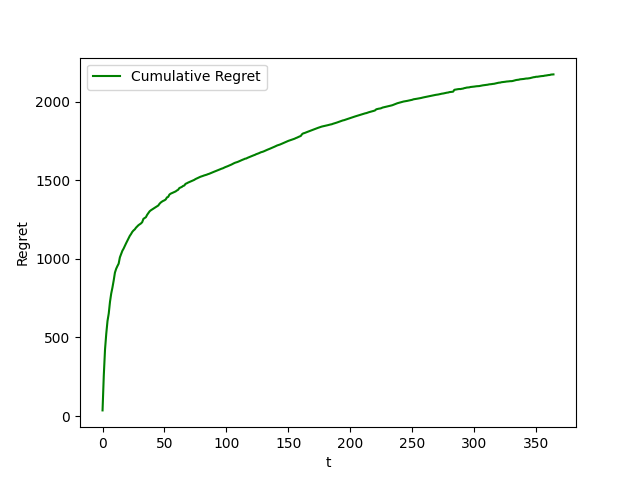
\includegraphics[width=0.8\textwidth]{images/assignment_2_cum_regret.png}
\caption{The cumulative regret shows a fast increase in the beginning, corresponding to a predominant exploration, and then slows down favoring the exploitation of the results.}
\end{figure}
\end{frame}

\begin{frame}{Assignment 2 - Instantaneous Regret}
\begin{figure}[hbtp]
\centering
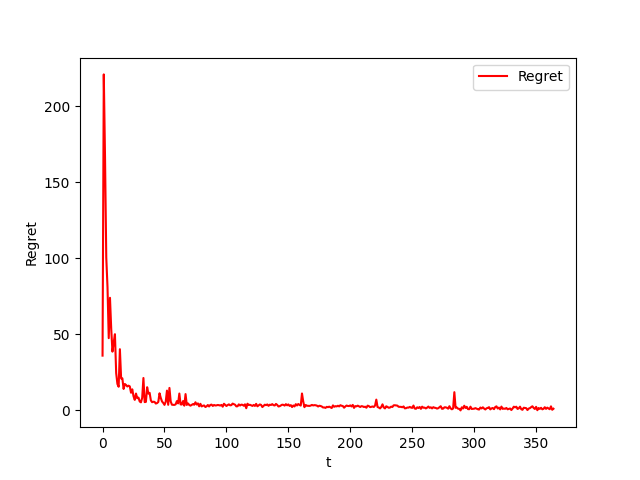
\includegraphics[width=0.8\textwidth]{images/assignment_2_regret.png}
\caption{The regret goes to 0 in approximately 50 steps.}
\end{figure}
\end{frame}

\begin{frame}{Assignment 3}
\textit{Design a sliding-window combinatorial bandit algorithm for the case, instead, in which there are the three phases aforementioned. Plot the cumulative regret and compare it with the cumulative regret that a non-sliding-window algorithm would obtain.}
\end{frame}

\begin{frame}[fragile]{Assignment 3 - Pseudocode}
\begin{lstlisting}
|\color{cyan}initialize| click envs
|\color{cyan}for| exp |\color{cyan}in| n_experiments:
  |\color{cyan}initialize| gp-ts and gp-ts-sw learners 
  |\color{cyan}for| t |\color{cyan}in| time_horizon:
  	|\color{cyan}if| abprupt_phase is changed:
  		|\color{cyan}reset| memory of the learners
    draw samples for each subcampaign
    find super-arm by solving knapsack problem
    |\color{cyan}pull| arms given by super-arm
    |\color{cyan}update| gp-ts and gp-ts-sw learners
|\color{cyan}calculate| clairvoyant value
|\color{cyan}plot| rewards and regrets for the 2 learners
\end{lstlisting}
\end{frame}

\begin{frame}{Assignment 3 - Experiments}
Setting \#1, \#2, \#3 parameters:
\begin{itemize}
\item T = 360
\item Number of arms = 21
\item Number of experiments = 25
\item Sliding window = 50, 90, 120
\end{itemize}
\end{frame}

\begin{frame}{Assignment 3 -  Cumulative Regret}
\begin{figure}[hbtp]
\centering
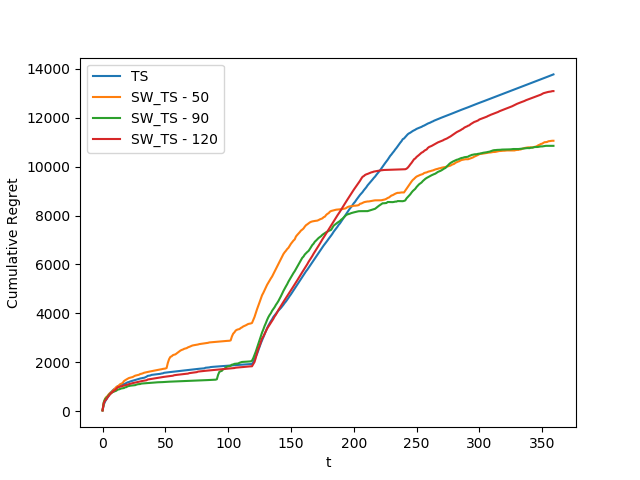
\includegraphics[width=0.8\textwidth]{images/assignment_3_exp_1_cum_regret.png}
\caption{All TS-SW settings perform better than the pure TS approach. Among them, the sliding window = 90 has the overall best performance.}
\end{figure}
\end{frame}

\begin{frame}{Assignment 3 - Rewards}
\begin{figure}[hbtp]
\centering
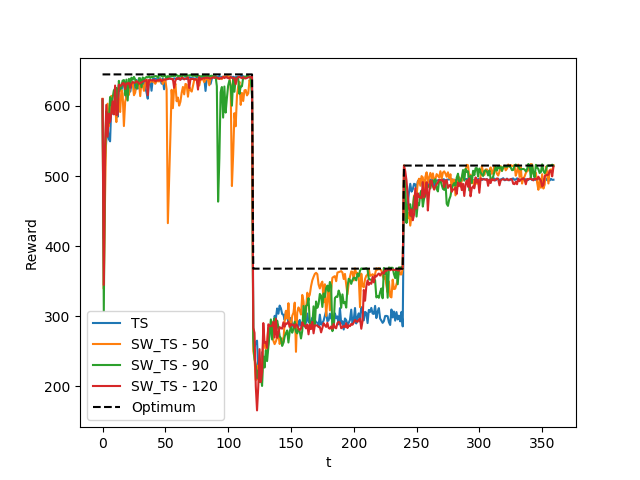
\includegraphics[width=0.8\textwidth]{images/assignment_3_exp_1_cum_reward.png}
\caption{This plot shows that the TS approach is unable to reach the optimal values in the second and third phases, while the sliding window = 90 always produces good results.}
\end{figure}
\end{frame}

\begin{frame}{Assignment 4}
\textit{Design a learning algorithm for pricing when the users that will buy the product are those that have clicked on the ads. Assume that the allocation of the budget over the three subcampaigns is fixed and there is only one phase (make this assumption also in the next steps). Plot the cumulative regret.}
\end{frame}

\begin{frame}[fragile]{Assignment 4 - Pseudocode}
\begin{lstlisting}
|\color{cyan}initialize| pricing envs
|\color{cyan}for| exp |\color{cyan}in| n_experiments:
  |\color{cyan}initialize| ts and greedy learners 
  |\color{cyan}for| t |\color{cyan}in| time_horizon:
    draw samples for each subcampaign (ts learner)
    |\color{cyan}update| ts learner
    draw samples for each subcampaign (greedy learner)
    |\color{cyan}update| greedy learner
|\color{cyan}calculate| clairvoyant value
|\color{cyan}plot| rewards and regrets for the 2 learners
\end{lstlisting}
\end{frame}

\begin{frame}{Assignment 4 - Experiments}
General parameters:
\begin{itemize}
\item Number of experiments = 50
\item User class probabilities = $[\frac{1}{5}, \frac{2}{5}, \frac{2}{5}]$
\end{itemize} 
Setting \#1, parameters:
\begin{itemize}
\item T = 365
\item Number of arms = $\ceil{(T \log{(T)})^{\frac{1}{4}}}$ = 8
\end{itemize}
Setting \#2, parameters:
\begin{itemize}
\item T = 365
\item Number of arms = $4 \times \ceil{(T \log{(T)})^{\frac{1}{4}}} = 32$
\end{itemize}
Setting \#3, parameters:
\begin{itemize}
\item T = 18250
\item Number of arms = $\ceil{(T \log{(T)})^{\frac{1}{4}}} = 23$
\end{itemize}
\end{frame}

\begin{frame}{Assignment 4 - Setting \#1, Regret}
\begin{figure}[hbtp]
\centering
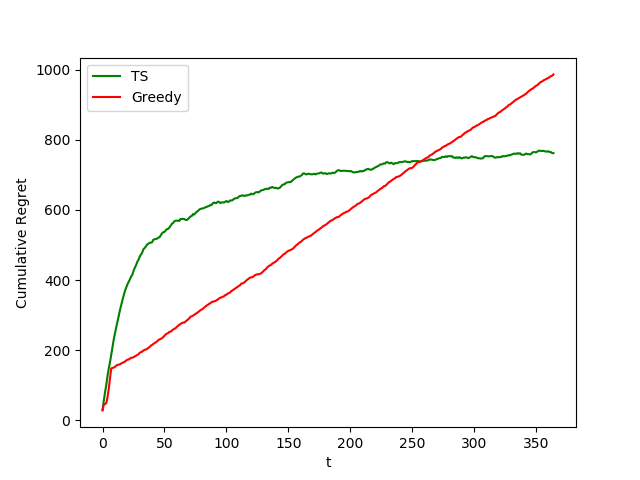
\includegraphics[width=0.8\textwidth]{images/assignment_4_exp_1_cum_regret.png}
\caption{Comparison of the cumulative regrets of a TS and a Greedy approach. The Greedy algorithm performs well at the beginning but loses in the end.}
\end{figure}
\end{frame}

\begin{frame}{Assignment 4 - Setting \#1, Reward}
\begin{figure}[hbtp]
\centering
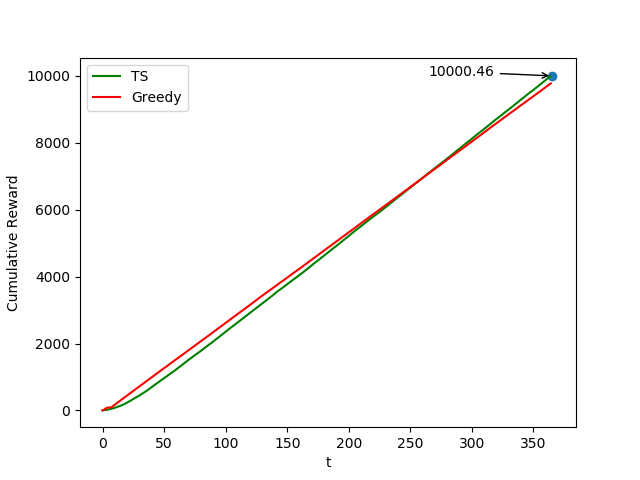
\includegraphics[width=0.8\textwidth]{images/assignment_4_exp_1_cum_reward.png}
\caption{Cumulative reward collected during the learning.}
\end{figure}
\end{frame}

\begin{frame}{Assignment 4 - Setting \#2, Regret}
\begin{figure}[hbtp]
\centering
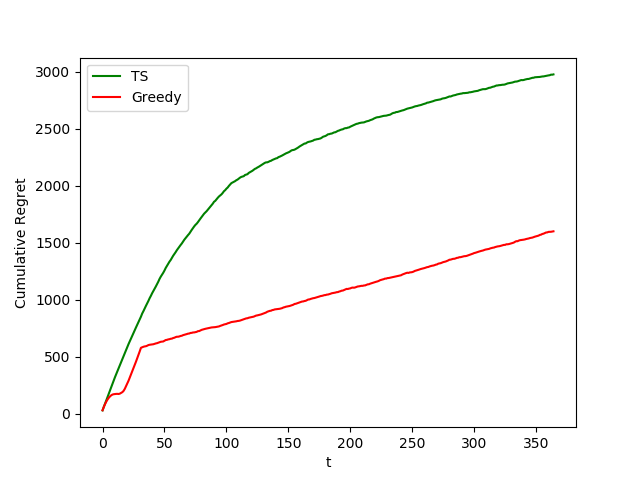
\includegraphics[width=0.8\textwidth]{images/assignment_4_exp_2_cum_regret.png}
\caption{This experiment shows that selecting a large number of candidates (4x than before) doesn't guarantee better results. The regret is more than tripled and the TS approach is performing worse than the Greedy one.}
\end{figure}
\end{frame}

\begin{frame}{Assignment 4 - Setting \#2, Reward}
\begin{figure}[hbtp]
\centering
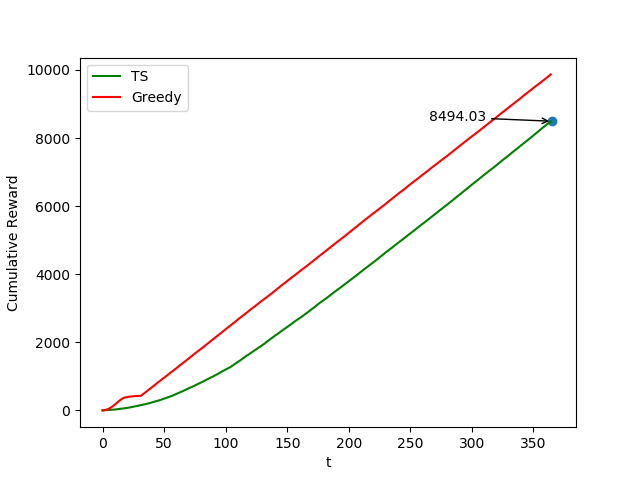
\includegraphics[width=0.8\textwidth]{images/assignment_4_exp_2_cum_reward.png}
\caption{Cumulative reward collected during the learning. The TS algorithm is significantly under the Greedy algorithm.}
\end{figure}
\end{frame}

\begin{frame}{Assignment 4 - Setting \#3, Regret}
\begin{figure}[hbtp]
\centering
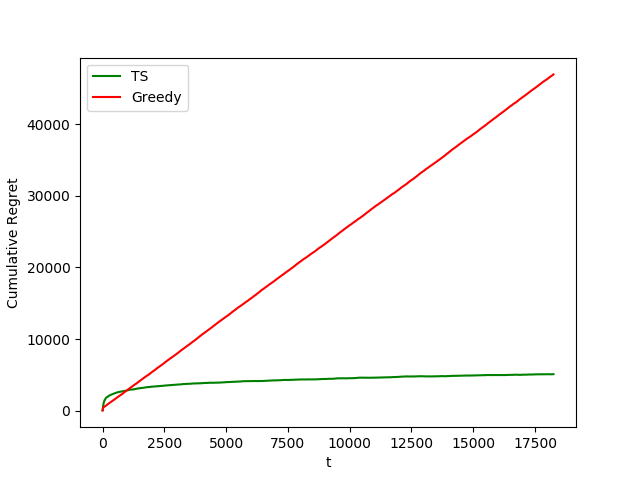
\includegraphics[width=0.8\textwidth]{images/assignment_4_exp_3_cum_regret.png}
\caption{This experiment aims to produce a reference for the results obtained with context generation in the \hyperlink{page.42}{next assignment}. The algorithm is launched for a number of steps = 50 (updates each day) $\times$ 365 (days) = 18250.}
\end{figure}
\end{frame}

\begin{frame}{Assignment 4 - Setting \#3, Reward}
\begin{figure}[hbtp]
\centering
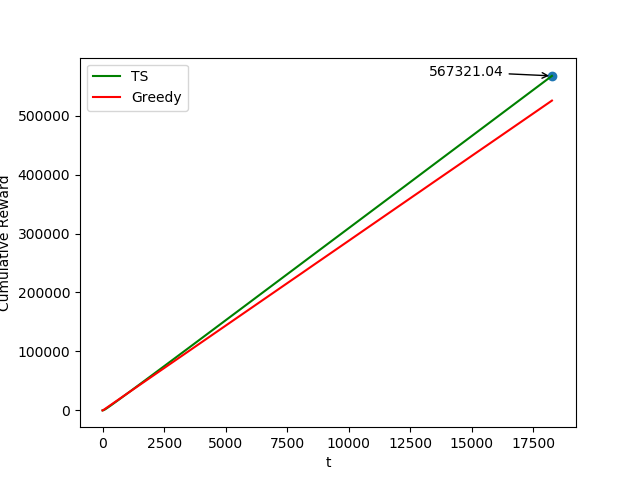
\includegraphics[width=0.8\textwidth]{images/assignment_4_exp_3_cum_reward.png}
\caption{Cumulative reward collected during the learning.}
\end{figure}
\end{frame}

\begin{frame}{Assignment 5}
\textit{Design and run a context generation algorithm for the pricing when the budget allocated to each single subcampaign is fixed. At the end of every week, use the collected data to generate contexts and then use these contexts for the following week. Plot the cumulative regret as time increases. In the next steps, do not use the generated contexts, but use all the data together.}
\end{frame}

\begin{frame}[fragile]{Assignment 5 - Pseudocode}
\begin{lstlisting}
|\color{cyan}initialize| pricing envs
|\color{cyan}for| exp |\color{cyan}in| n_experiments:
  |\color{cyan}initialize| context generator 
  |\color{cyan}for| t |\color{cyan}in| time_horizon:
    |\color{cyan}if| trimester is ended:
      |\color{cyan}generate| new contexts (greedy approach)
    |\color{cyan}for| context |\color{cyan}in| n_contexts:
      |\color{cyan}run| ts algorithm
|\color{cyan}calculate| clairvoyant value
|\color{cyan}plot| rewards and regrets
\end{lstlisting}
\end{frame}

\begin{frame}{Assignment 5 - Experiments}
Setting \#1, parameters:
\begin{itemize}
\item T = 18250
\item Number of arms = $\ceil{(T \log{(T)})^{\frac{1}{4}}}$ = 23
\item User class probabilities = $[\frac{1}{5}, \frac{2}{5}, \frac{2}{5}]$
\item Number of experiments = 50
\end{itemize}
\end{frame}

\begin{frame}{Assignment 5 - Cumulative Regret}
\begin{figure}[hbtp]
\centering
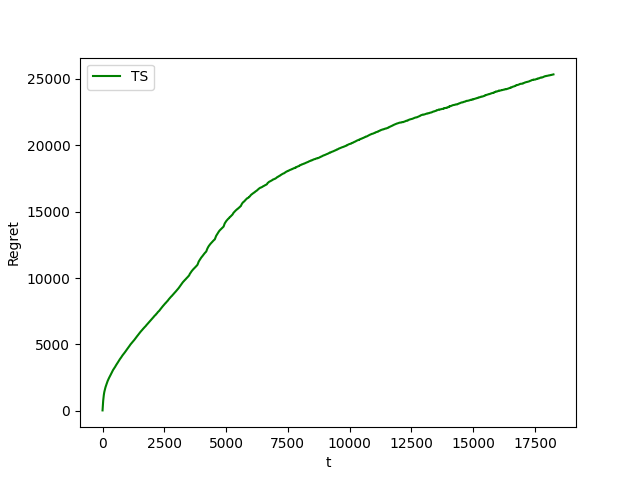
\includegraphics[width=0.8\textwidth]{images/assignment_5_cum_regret.png}
\caption{If we compare this result with the one obtained in \hyperlink{page.37}{assignment 4}, we can see that we obtain a worse result in terms of cumulative regret, but this is due to the method that we use to compute the optimum in the two cases.}
\end{figure}
\end{frame}

\begin{frame}{Assignment 5 - Cumulative Reward}
\begin{figure}[hbtp]
\centering
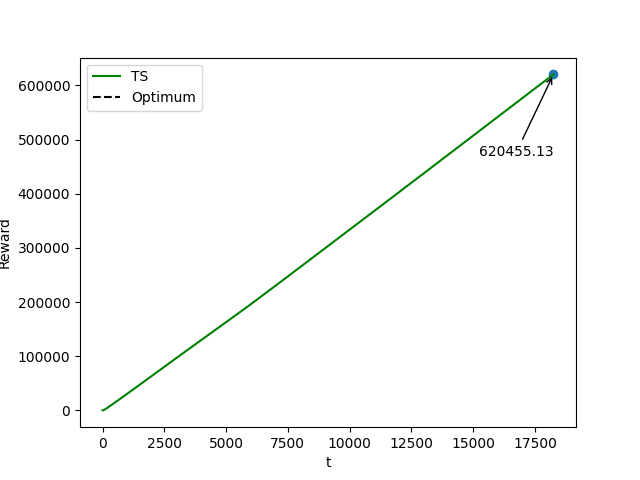
\includegraphics[width=0.8\textwidth]{images/assignment_5_reward.png}
\caption{If we look instead to the cumulative reward, we can see that we get a better result compared to assignment 4 (573k vs 567k). }
\end{figure}
\end{frame}

\begin{frame}{Assignment 6}
\textit{Design an optimization algorithm combining the allocation of budget and the pricing when the seller a priori knows that every subcampaign is associated with a different context and charges a different price for every context. Suggestion: the value per click to use in the knapsack-like problem depends on the pricing, that depends on the number of users of a specific class interested in buying the product. Notice that the two problems, namely, pricing and advertising, can be decomposed since each subcampaign targets a single class of users, thus allowing the computation of the value per click of a campaign only on the basis of the number of clicks generated by that subcampaign. Plot the cumulative regret when the algorithm learns both the conversion rate curves and the performance of the advertising subcampaigns.}
\end{frame}

\begin{frame}{Assignment 6 - Experiment}
\begin{itemize}
\item T = 365
\item Number of experiments = 50
\item Class probabilities = \( \left[ \frac{1}{4}, \frac{1}{2}, \frac{1}{4} \right] \)
\item Number of arms pricing = $\ceil{(T \log{(T)})^{\frac{1}{4}}}$ = 8
\item Number of arms advertising = 21
\end{itemize}
\end{frame}

\begin{frame}[fragile]{Assignment 6 - Pseudocode}
\begin{lstlisting}
|\color{cyan}|
|\color{cyan}initialize| pricing and click envs
|\color{cyan}for| exp |\color{cyan}in| n_experiments:
	|\color{cyan}initialize| ts and gp-ts learners 
	|\color{cyan}for| t |\color{cyan}in| time_horizon:
		|\color{cyan}for| s |\color{cyan}in| subcampaign:
			draw a (price, conversion_rate) sample with ts		learner
			get return from the pricing env, given the price
			update ts learner
			draw click samples with gp-ts learner
			weight the clicks with price and conversion_rate	previously selected by the ts learner
		find super-arm by solving knapsack problem
		get revenues = clicks * price * conversion_rate from the click envs by pulling the super-arm
		|\color{cyan}update| gp-ts learners 
|\color{cyan}calculate| clairvoyant value
|\color{cyan}plot| rewards and regrets
\end{lstlisting}
\end{frame}

\begin{frame}{Assignment 6 - Cumulative Regret}
\begin{figure}[hbtp]
\centering
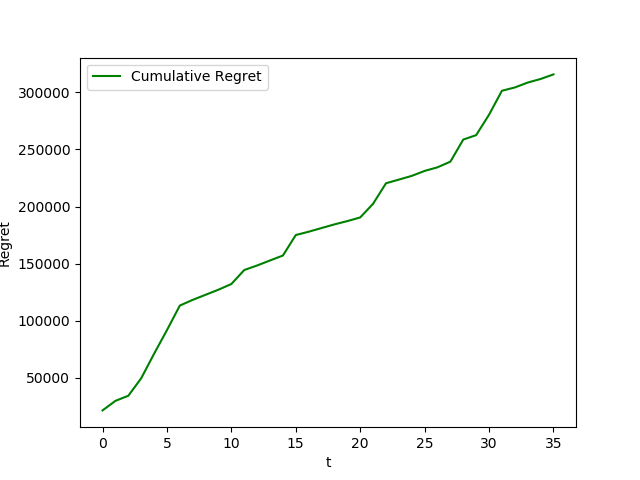
\includegraphics[width=0.8\textwidth]{images/assignment_6_cum_regret.png}
\caption{Analyzing the cumulative regret of the algorithm we can observe that the curve has almost an asymptotic progress meaning that the algorithm is almost near to the optimal solution.}
\end{figure}
\end{frame}

\begin{frame}{Assignment 6 - Cumulative Reward}
\begin{figure}[hbtp]
\centering
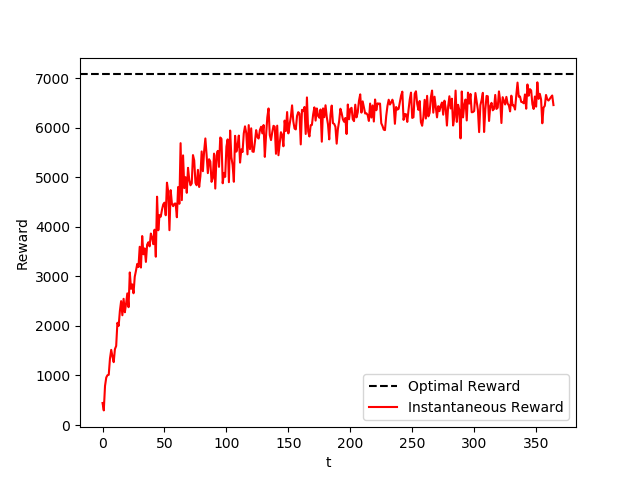
\includegraphics[width=8cm]{images/assignment_6_inst_reward.png}
\caption{If instead we observe the instantaneous reward, we can see that the algorithm is almost near to reach the optimal value.}
\end{figure}
\end{frame}

\begin{frame}{Assignment 7}
\textit{Do the same of Step 6 under the constraint that the seller charges a unique price to all the classes of users. Suggestion: for every possible price, fix this price and repeat the algorithm used in Step 6. Plot the cumulative regret when the algorithm learns both the conversion rate curves and the performance of the advertising subcampaigns.}
\end{frame}

\begin{frame}{Assignment 7 - Experiment}
\begin{itemize}
\item T = 365
\item Number of experiments = 15
\item Class probabilities = \( \left[ \frac{1}{4}, \frac{1}{2}, \frac{1}{4} \right] \)
\item Number of arms pricing = $\ceil{(T \log{(T)})^{\frac{1}{4}}}$ = 8
\item Number of arms advertising = 21
\end{itemize}
\end{frame}

\begin{frame}[fragile]{Assignment 7 - Pseudocode}
\begin{lstlisting}
|\color{cyan}|
|\color{cyan}initialize| pricing and click envs
|\color{cyan}for| exp |\color{cyan}in| n_experiments:
	|\color{cyan}for| price |\color{cyan}in| n_prices:
		|\color{cyan}initialize| ts and gp-ts learners 
		|\color{cyan}for| t |\color{cyan}in| time_horizon:
			|\color{cyan}for| s |\color{cyan}in| subcampaign:
				|\color{cyan}select| current price and conversion_rate 
				get return from the pricing env, given the				price
				|\color{cyan}update| ts learner
				draw click samples with gp-ts learner
				weight the clicks with price and                   conversion_rate previously selected
			find super-arm by solving knapsack problem
			|\color{cyan}collect| revenues = = clicks * price *             conversion_rate from the click envs by pulling    the super-arm
			|\color{cyan}update| gp-ts learners 
|\color{cyan}calculate| clairvoyant value
|\color{cyan}plot| rewards and regrets
\end{lstlisting}
\end{frame}

\begin{frame}{Assignment 7 - Regrets of optimal arm}
\begin{figure}[hbtp]
\centering
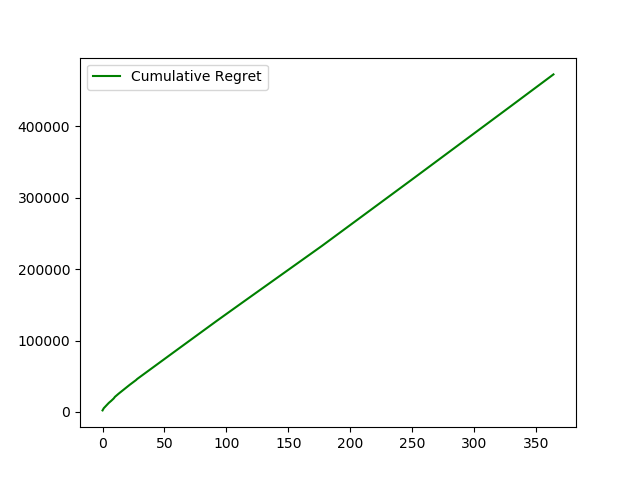
\includegraphics[width=0.8\textwidth]{images/assignment_7_regrets_arm_3_cum_regret.png}
\caption{The slope of the curve shows an initial phase of learning and exploration that is stopped from 3 phases of suboptimal solutions in which the regret increases linearly.}
\end{figure}
\end{frame}

\begin{frame}{Assignment 7 - Rewards of optimal arm}
\begin{figure}[hbtp]
\centering
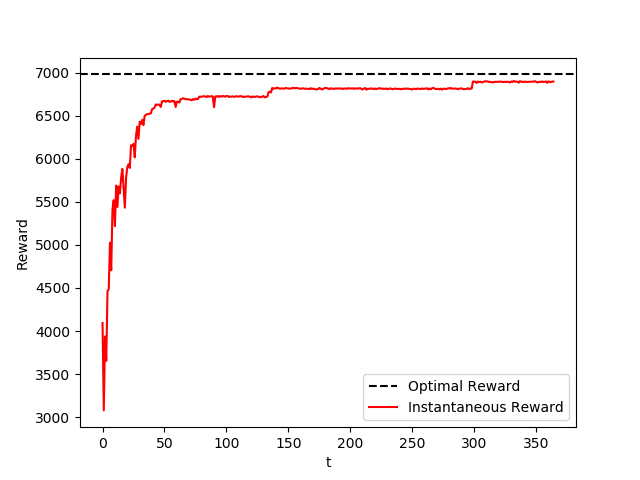
\includegraphics[width=0.8\textwidth]{images/assignment_7_regrets_arm_3_inst_reward.png}
\caption{Here we can notice that the algorithm reaches a stable point near the optimum but cannot manage to increase its value.}
\end{figure}
\end{frame}

\begin{frame}{Assignment 6 \& 7 Comparison}
	\begin{itemize}
		\item Optimal value:
		\begin{itemize}
			\item Assignment 6: 7074
			\item Assignment 7: 6977
		\end{itemize}
		The difference between the two is due to the imposed price of the assignment 7.
		\item Assignment 6 shows a slower a increase of instant reward while assignment 7 reaches high values quite immediately. Responsibility lies with the exploration phase of assignment 6 that tries more different prices while assignment 7 has only one imposed price.
	\end{itemize}
\end{frame}

\begin{frame}{Assignment 6 \& 7 Comparison}
	\begin{itemize}
		\item Assignment 6 shows a bigger cumulative regret than the one of assignment 7. This can be justified by the initial exploration phase in which a lot of regret is accumulated.
		\item Assignment 6 has a continuously decreasing slope of cumulative regret while assignment 7 shows a quite linear slope, this underlines that assignment 6 is improving while assignment 7 has settled in a sub-optimal solution.
	\end{itemize}
\end{frame}

\end{document}